\documentclass[oneside, 11pt]{book}

\usepackage[a-1b]{pdfx}

\usepackage[subpreambles=false]{standalone}
\usepackage{import}
\usepackage{minitoc}
\usepackage{breakcites}
\usepackage[a4paper, 
            left=3cm, 
            right=2cm, 
            top=2cm, 
            bottom=2cm]{geometry}
\usepackage{emptypage}
\usepackage{fancyhdr}
\pagestyle{fancy}


% fancy heading settings for chapter contents
\renewcommand{\chaptermark}[1]{\markboth{{\thechapter.\ #1}}{}}
\renewcommand{\sectionmark}[1]{\markright{\thesection.\ #1}}
\fancyhead[R]{\thepage}
\fancyhead[L]{\leftmark}
\fancyfoot{}

\usepackage[nobreak]{mdframed} % do not break example across pages
\usepackage{lipsum}

% set color for links, urls and cites
\hypersetup{
    breaklinks,
    colorlinks=true,
    linkcolor=.,
    urlcolor=.,
    citecolor=teal
}
% captions setup
\usepackage{caption}
\usepackage{subcaption}
\captionsetup{justification=raggedright,singlelinecheck=false} % make captions left-aligned
\captionsetup[figure]{labelfont={bf},name={Fig.},labelsep=period, font=footnotesize} % Use Fig. instead of Figure in captions
\renewcommand{\figureautorefname}{Fig.} % Redefine autoref name for figures
% for strikethrough
\usepackage{soul}
\setstcolor{grey}
% for inserting pdfs
\usepackage[demo]{pdfpages} % puts an empty page instead of study PDFs. This should be used for submission and printing of thesis
% \usepackage{pdfpages} % uncomment to put the actual PDFs
% smart and nestable quote marks
\usepackage{csquotes}
% line spacing
\usepackage{setspace}
\setstretch{1.15}
% \setlength{\parindent}{0pt} % Remove paragraph indentation (optional)
% set first level bullet points to dash
\renewcommand\labelitemi{-}

% useful tools for the drafting/editing process
% for inline or PDF comments
\usepackage{todonotes}
% Add comments as pdf comments (comment out to use inline/side) comments
% \usepackage{pdfcomment} % To enable PDF annotations
\usepackage{xparse}
\RenewDocumentCommand{\todo}{O{} m}{\pdfcomment[color=yellow, author=Amin]{#2}}
% for highlighting changes
\usepackage{changes}

% for chapter title spacing
\usepackage{titlesec}
% \titleformat{\chapter}[display]   
% {\normalfont\huge\bfseries}{\chaptertitlename\ \thechapter}{20pt}{\Large}
% \titlespacing*{\chapter}{0pt}{0pt}{40pt}

% setting the depth for section numbering
\setcounter{secnumdepth}{3}

%%% Citations setup %%%
% While drafting the following command can be used to put temporary citation placeholders
\newcommand{\citetemp}[1]{[#1]}
% But to put actual citations we'll need a `.bib` file including all the citations
% (here named `example.bib`)
% To create this file I recommend using Zotero with "Better BibTeX" plugin by:
% 1. In Better BibTeX settings, ignore fields "note,rights,copyright,langid,keywords,file,month,urldate,issn,abstract". Also “When an item has both …” → select DOI.
% 2. Put all your thesis references in a subcollection
% 3. Right click on the subcollection and select "Export Collection...", then export the library as “Better BibTex” (not BibLaTex) 
% 4. If you've been using `\citetemp` in the document, replace `\citetemp` calls with `\cite`
% 5. We need the following to set up bibliography in LaTeX
\usepackage[
backend=biber,
style=apa,
]{biblatex}
\addbibresource{example.bib} % replace with the name of your `.bib` file

\begin{document}

%%%%%%%%%%%%%%%%%%%% Front Matter
\frontmatter
% title page
\import{frontmatter}{titlepage}
\clearpage
% committee details; comment this out for the thesis submission. This page is only needed for the printed version submitted to the library after defence.
\import{frontmatter}{committee}
\clearpage
% dedications / quote; optional
\import{frontmatter}{dedications}
\clearpage
% list of publications included in thesis
\import{frontmatter}{publications}
\clearpage

\setcounter{page}{1} % start page numbers from abstract
% make chapter titles invisible
\titleformat{\chapter}[display]{\Huge\bfseries}{}{0pt}{}
\titlespacing*{\chapter}{0pt}{-5em}{0pt}

% German and English abstracts
\chapter*{}
\setstretch{1.10} % temporarily decrease line spacing to fit german abstract in one page
\import{frontmatter}{zusammenfassung}
\setstretch{1.15} % reset line spacing
\chapter*{}
\import{frontmatter}{abstract}

% abbreviations
\chapter*{}
\import{frontmatter}{abbreviations}

%%%%%%%%%%%%%%%%%%%% TOC
% reset chapter title formatting
\titleformat{\chapter}[display]
  {\LARGE\bfseries}                % Overall chapter format (default)
  {\chaptername\ \thechapter}      % Formatting for "Chapter X" (Number)
  {14pt}                           % Space between number and title
  {\huge\bfseries}                % Formatting for chapter title
\titlespacing*{\chapter}{0pt}{0pt}{40pt}
\dominitoc
\tableofcontents

%%%%%%%%%%%%%%%%%%%%
\mainmatter
%%%%%%%%%%%%%%%%%%%% Main matter
\setlength{\parskip}{1em} % Add space between paragraphs

\chapter{Introduction}\label{chap:intro}
\import{intro}{intro} % imports "intro/intro.tex"

\chapter{Study 1: Title}\label{chap:study1}
\import{study1}{study1} % imports "study1/study1.pdf" which is the paper PDF (in journal format)
% Store current page number and include the PDF
\newcounter{tempPage} % Temporary counter to store page number
\setcounter{tempPage}{\value{page}} % Store current page number
\clearpage
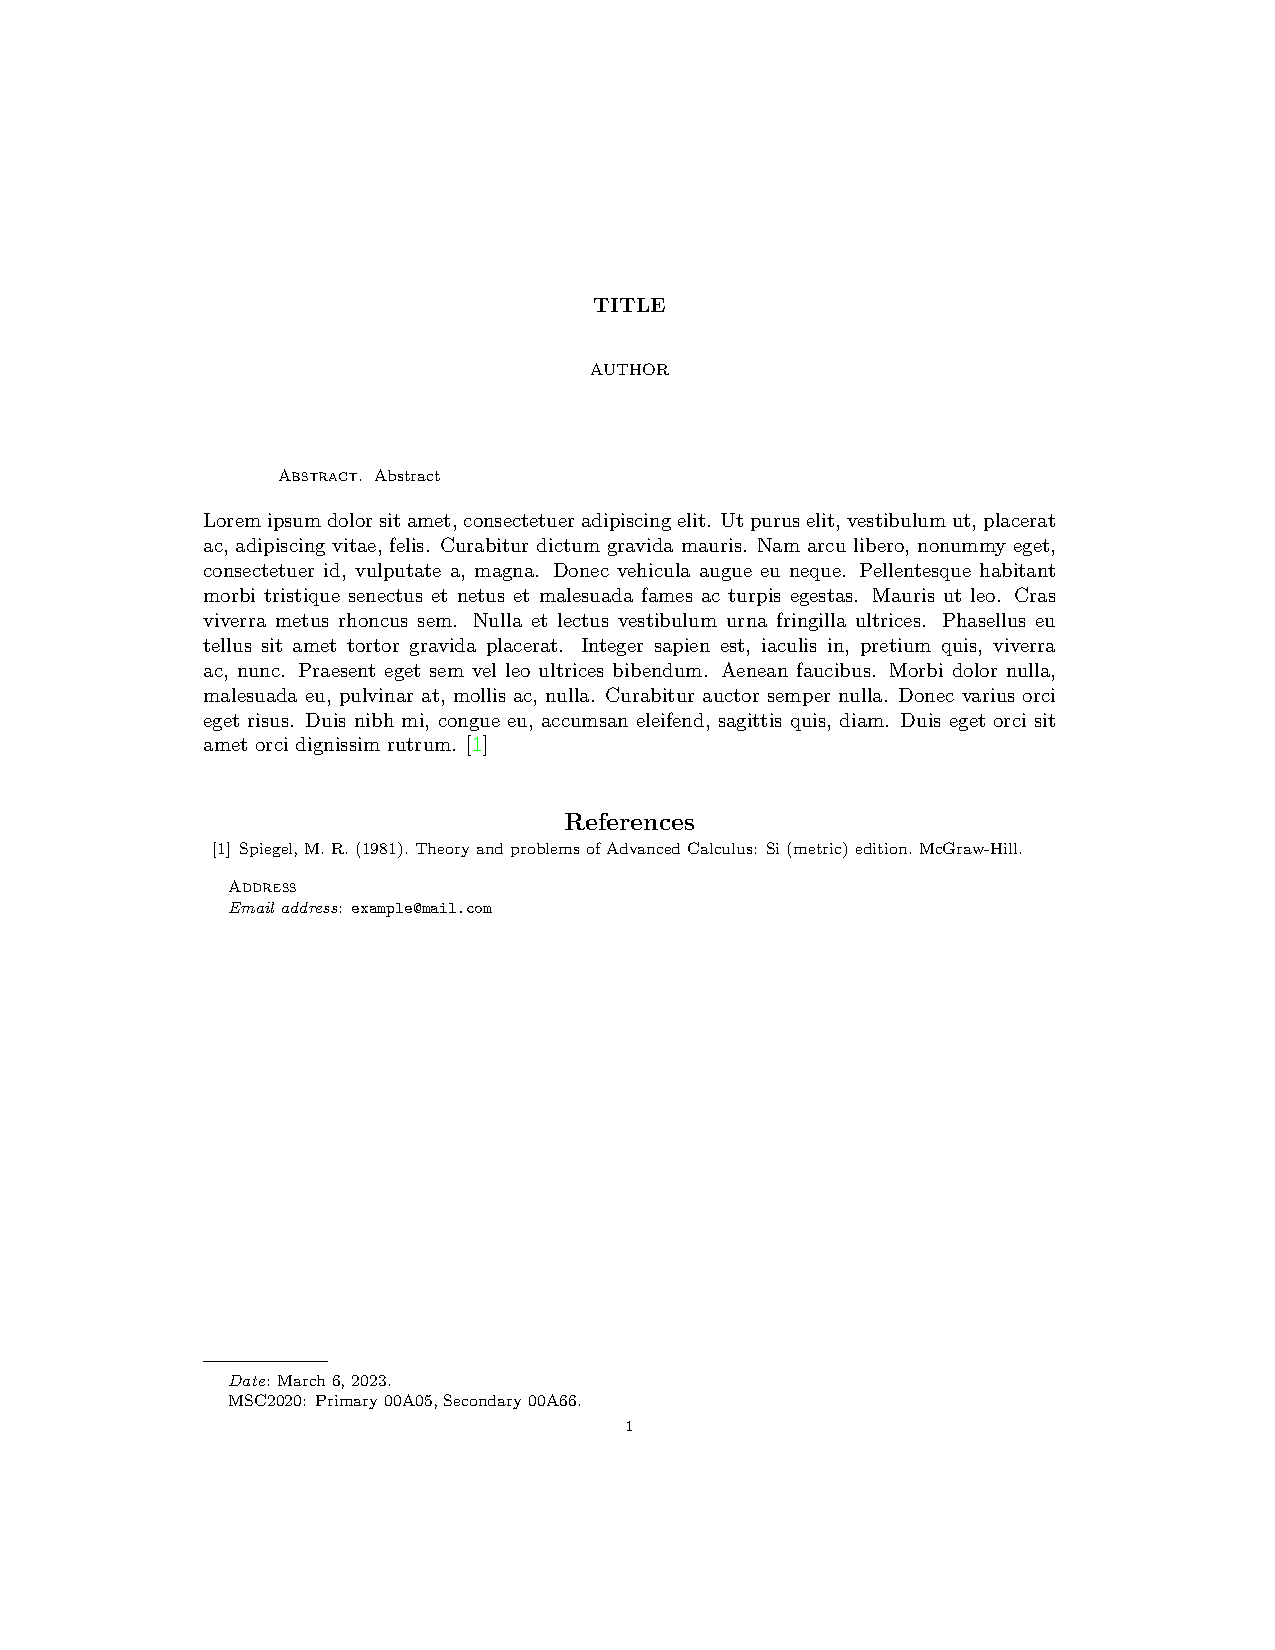
\includepdf[pages=-, fitpaper=false, pagecommand={\thispagestyle{empty}}, frame=true, scale=0.9]{study1/study1.pdf}
\setcounter{page}{\value{tempPage}} % Restore the page number
\addtocounter{page}{1} % Increment the page number by 1

\chapter{Study 2: Title}\label{chap:study2}
\import{study2}{study2} % imports "study2/study2.pdf" which is the paper PDF (in journal format)
% Store current page number and include the PDF
\setcounter{tempPage}{\value{page}} % Store current page number
\clearpage
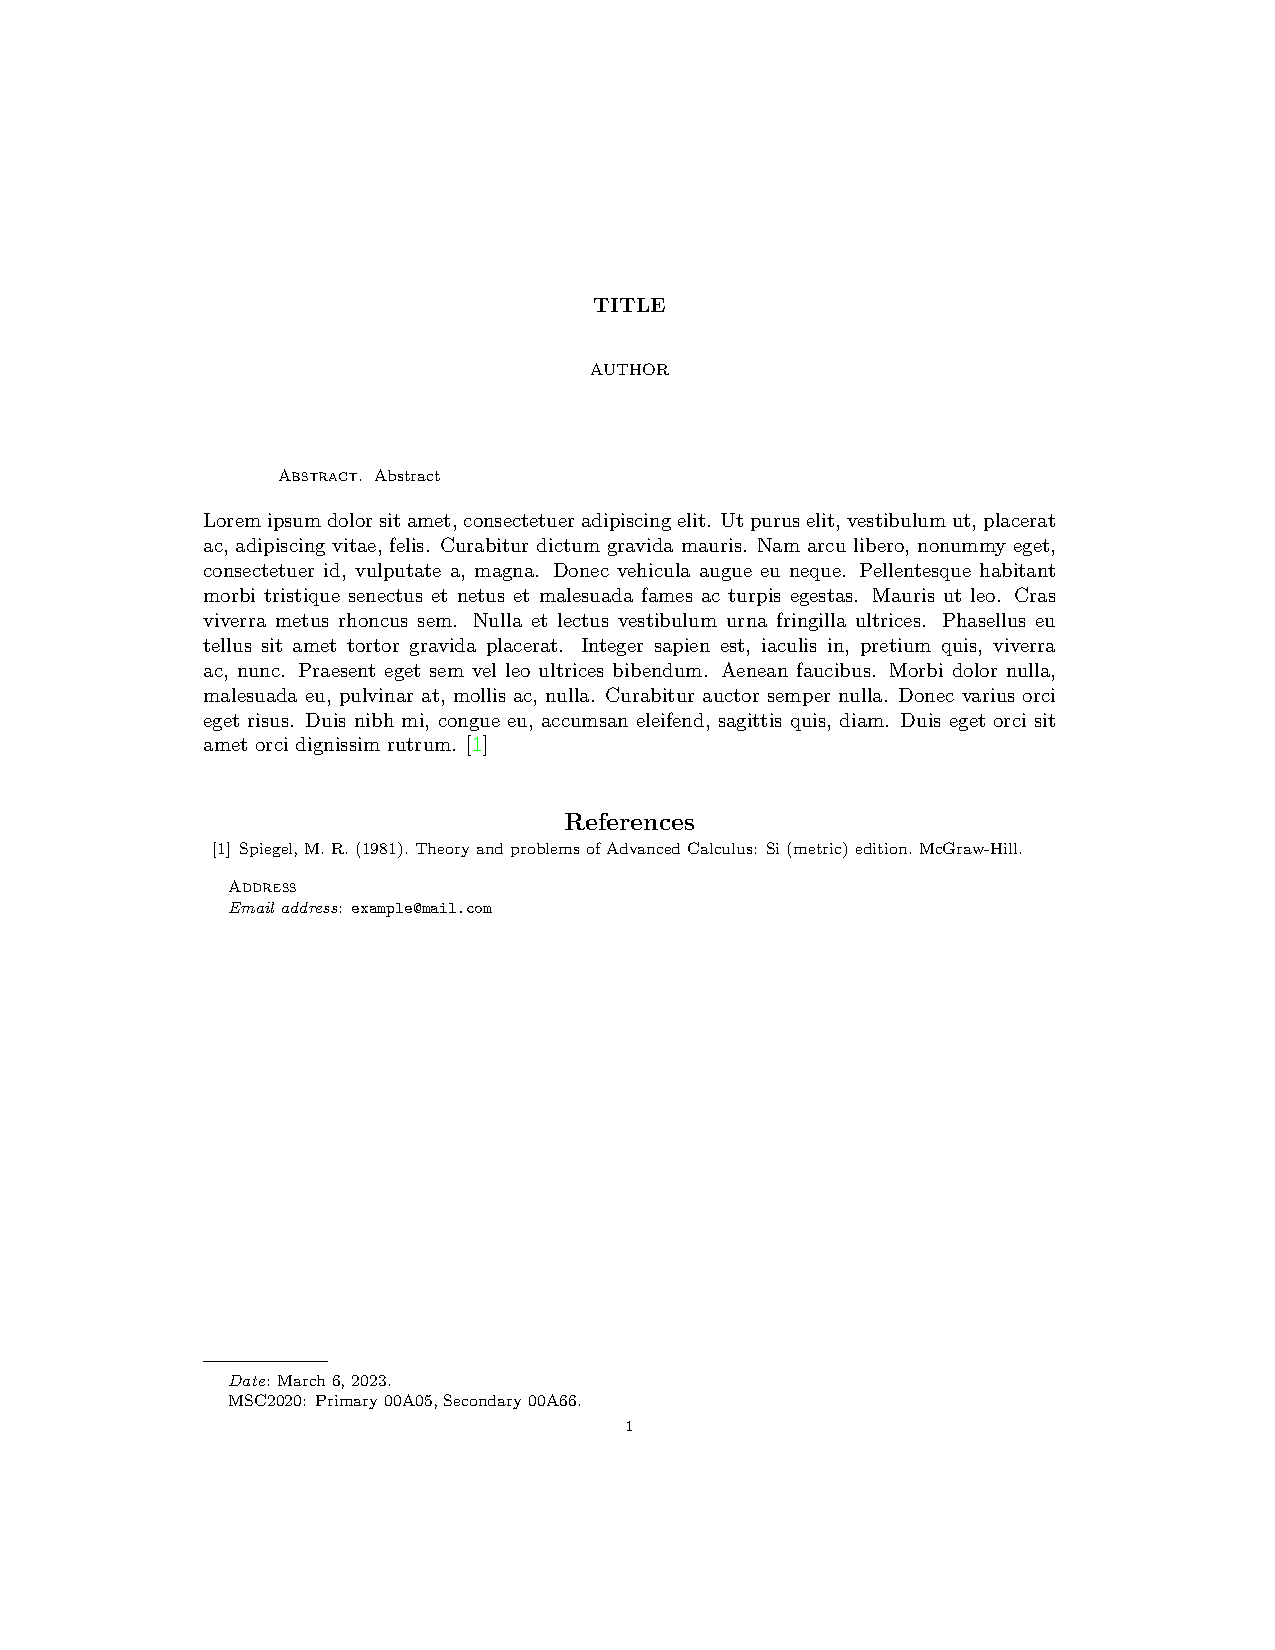
\includepdf[pages=-, fitpaper=false, pagecommand={\thispagestyle{empty}}, frame=true, scale=0.9]{study2/study2.pdf}
\setcounter{page}{\value{tempPage}} % Restore the page number
\addtocounter{page}{1} % Increment the page number by 1

\chapter{Study 3: Title}\label{chap:study3}
% \minitoc
\import{study3}{study3} % imports "study2/study2.pdf" which is the paper PDF (in journal format)
% Store current page number and include the PDF
\setcounter{tempPage}{\value{page}} % Store current page number
\clearpage
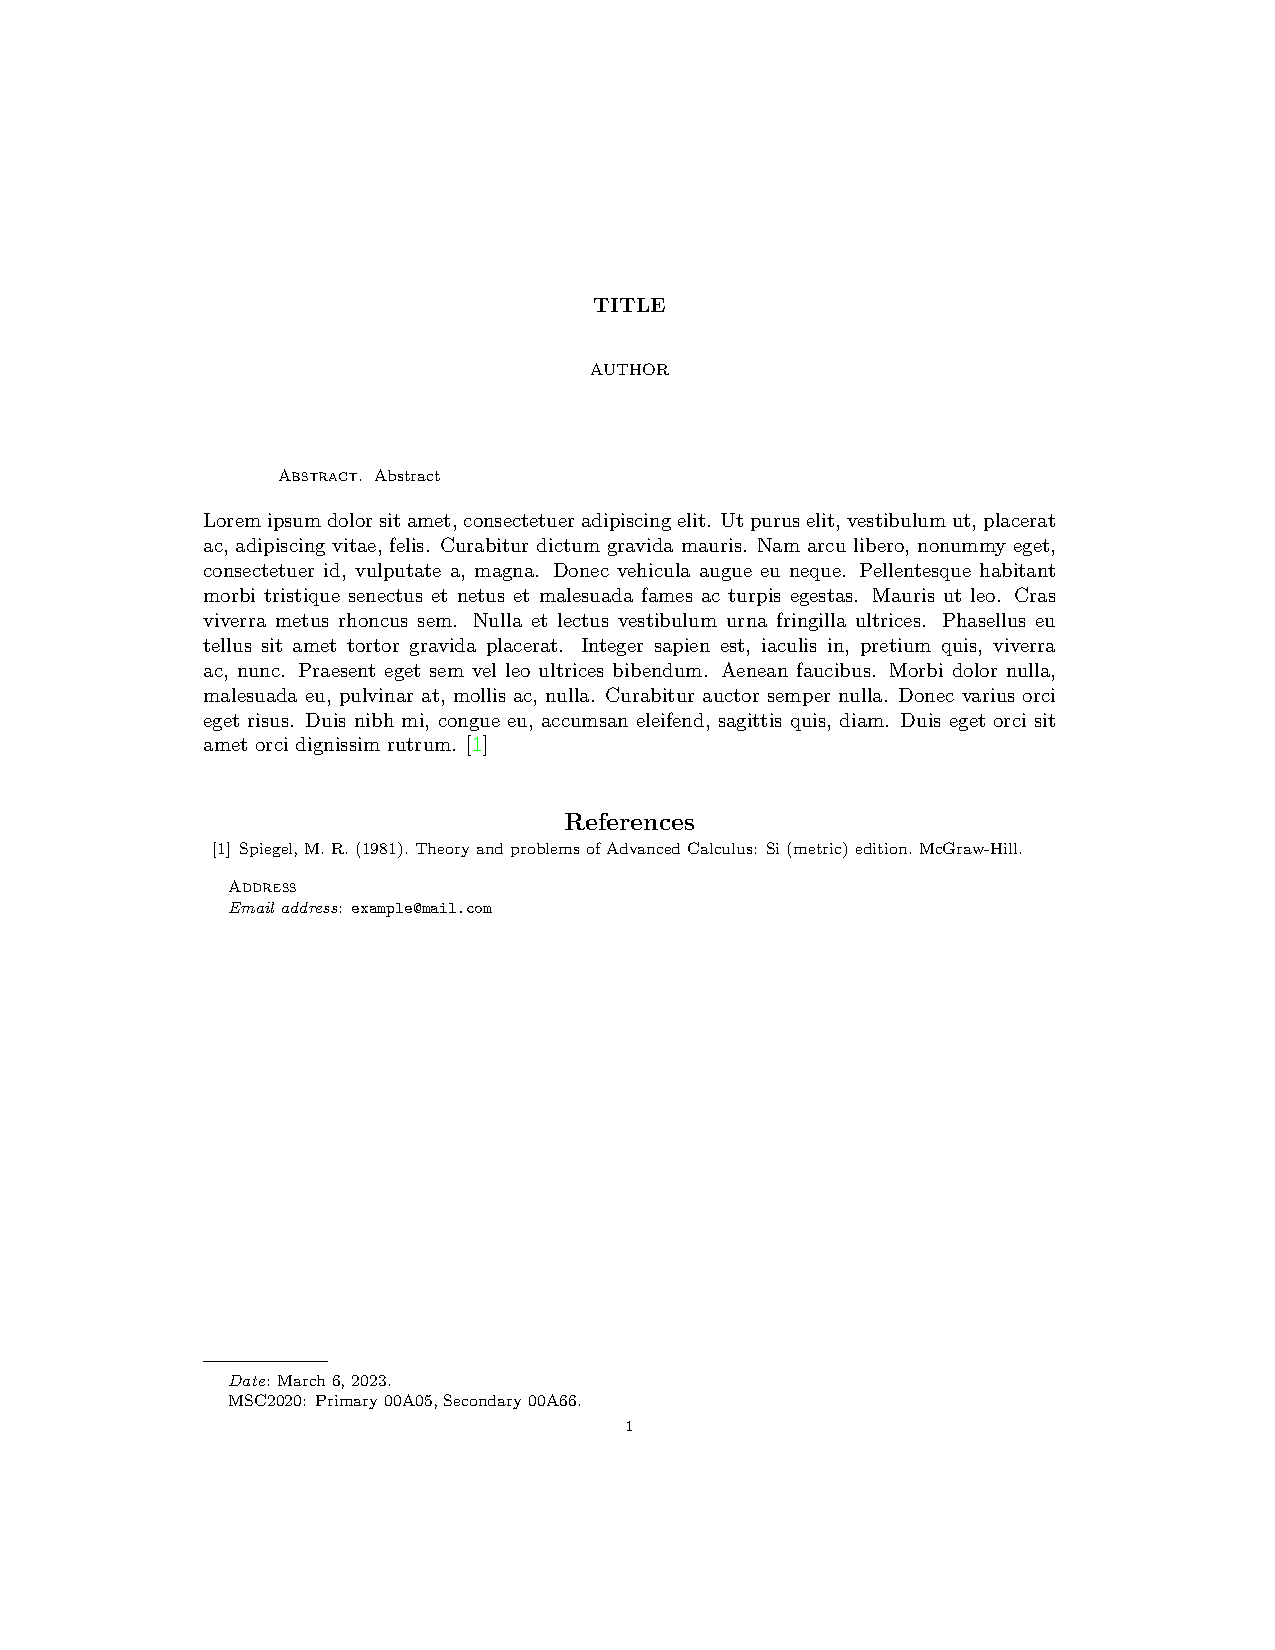
\includepdf[pages=-, fitpaper=false, pagecommand={\thispagestyle{empty}}, frame=true, scale=0.9]{study3/study3.pdf}
\setcounter{page}{\value{tempPage}} % Restore the page number
\addtocounter{page}{1} % Increment the page number by 1

\chapter{Discussion}\label{chap:discussion}
\import{discussion}{discussion} % imports "discussion/discussion.tex"

%%%%%%%%%%%%%%%%%%%%
\backmatter
%%%%%%%%%%%%%%%%%%%% Back matter
\cleardoublepage
\phantomsection
\addcontentsline{toc}{chapter}{Bibliography}
\printbibliography[title={Bibliography},prenote={\markboth{Bibliography}{Bibliography}}]

\cleardoublepage
\phantomsection
\addcontentsline{toc}{chapter}{Acknowledgments}\label{chap:acknowledgments}
\markboth{Acknowledgments}{Acknowledgments}
\import{ackn}{ackn}

\end{document}
